\section{ONF TR-512 - Modelul informaţional de bază (\textit{Core Model})}

Modelul informațional de bază (\textit{CoreModel}) reprezintă o recomandare tehnică făcută de grupul de Modelare Informaţională (\textit{Information Modeling}) din cadrul \gls{onf}. Aceasta propune un model care să descrie resursele din planul de date al unei rețele de transport, indiferent de tehnologia folosită, cu scopul de a fi folosit în activitățile de control și administrare.

Un model informațional descrie elementele dintr-un domeniu, în ceea ce priveşte obiectele, proprietăţile lor (reprezentate prin atribute) și relaţiile dintre acestea \cite{onftr512v1.0}. Scopul dezvoltării unui astfel de model este acela de a fi folosit de către echipamentele de control \gls{sdn}, pentru administrarea automată a unor astfel de rețele de transport, în concordanţă cu arhitectura \gls{sdn}. Echipamentul de control va prezenta cu ajutorul acestui model viziunea sa asupra rețelei către clienţii acestuia (care pot fi aplicații software sau alte echipamente de control).

Modelul informațional de bază propune un set de obiecte de bază care reprezintă planul de date al unei rețele, care sunt însă independente de tehnologia folosită pentru transportul datelor. Acestea pot fi apoi folosite pentru dezvoltarea de modele informaționale specifice pentru anumite tehnologii (de exemplu tehnologii fără fir - microunde sau unde milimetrice, tehnologii optice, etc.). Modelul conţine și obiecte care pot fi folosite în aplicații specifice, însă toate acestea sunt independente de protocoalele care ar putea fi folosite în planul de control. El este propus în limbajul \gls{uml} și se bazează și pe alte modele informaționale, propuse de alte organizaţii care dezvoltă standarde.

O imagine de ansamblu simplificată, folosind \gls{uml} se poate vedea în Figura \ref{fig:core_model}. Blocurile relevante pentru simulatoarele dezvoltate vor fi detaliate în paragrafele următoare. Nu se vor detalia toate obiectele care alcătuiesc modelul informațional de bază deoarece, așa cum este sugerat în recomandarea \gls{onf}, modelul poate fi redus și simplificat, în funcție de nevoile pentru care este folosit.  

\begin{figure}[h]
	\centering
	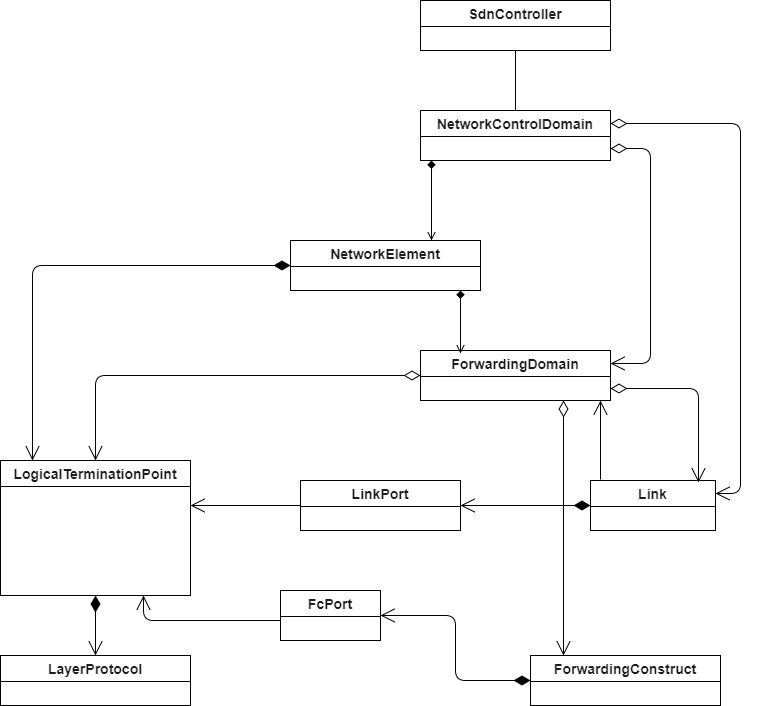
\includegraphics[width=1\textwidth]{core_model_uml_overview}
	\caption{Reprezentare UML simplificată a \textit{CoreModel} \cite{onftr512v1.2}.}
	\label{fig:core_model}
\end{figure}

\subsection{Obiectul Element de Rețea (\textit{NetworkElement - NE})}
%\paragraph{Network Element}

Obiectul \textit{Element de Rețea} - \gls{ne} - reprezintă un dispozitiv de rețea, adică, în cazul \gls{sdn}, un echipament de dirijare din planul de date, sau, în cazul în care există virtualizare, un element virtual de rețea vizibil de către interfaţa care folosește acea virtualizare.

Pentru o interfață directă de la echipamentul de control \gls{sdn} către un echipament de rețea, obiectul \textit{\gls{ne}} delimitează domeniul de control pentru resursele echipamentului, specificând funcții cum ar fi încapsularea folosită, multiplexarea, demultiplexarea, funcțiile asociate operaţiilor de administrare și de mentenanţă, etc. De asemenea, obiectul \textit{\gls{ne}} defineşte domeniul spaţiilor de adresare pentru identificarea obiectelor care reprezintă resursele conţinute de echipamentul respectiv.

În cazul în care se folosesc metode de virtualizare, obiectul \textit{NetworkElement} reprezintă un element virtual de rețea. Asocierea unui element virtual cu unul real este responsabilitatea echipamentului de control \gls{sdn}. Cu ajutorul interfeţei de Sud acesta poate crea sau şterge în mod dinamic astfel de obiecte pentru a oferi diferite imagini asupra rețelei, în funcție de nevoile aplicațiilor care se află deasupra echipamentului de control.

\subsection{Obiectele Punct Logic de Terminație (\textit{LogicalTerminationPoint - LTP}) și Nivelul Protocolului (\textit{LayerProtocol - LP})}

Obiectul \textit{Punct Logic de Terminație - \gls{ltp}} - cuprinde terminaţiile, adaptările sau funcțiile asociate operaţiilor de administrare și de mentenanţă ale unuia sau mai multor niveluri de transport. Prin natura sa, acest obiect suportă toate tipurile de protocoale, inclusiv cele pentru comutare de pachete sau pentru comutare de circuite. Fiecare nivel de transport este reprezentat de o instanţă a unui obiect de tip \textit{Nivelul Protocolului - \gls{lp}} -, instanţă care poate fi folosită pentru a controla terminaţiile sau funcțiile de administrare și mentenanţă ale nivelului respectiv, sau pentru adaptarea (încapsularea sau multiplexarea semnalului client).

Dacă relaţia client-server între resursele echipamentului reprezentate de obiectele \textit{\gls{ltp}} și \textit{\gls{lp}} are un grad de asociativitate de 1:1 și este imuabilă, atunci un obiect \textit{\gls{ltp}} poate conţine mai multe obiecte \textit{\gls{lp}}, de niveluri diferite de transport. Altfel, obiectele \textit{\gls{lp}} de pe niveluri diferite trebuie să aibă asociate obiecte \textit{\gls{ltp}} diferite.

Scopul acestor obiecte este acela de a oferi suport din perspectiva controlului și a administrării fără a fi nevoie de a defini atribute specifice unei anumite tehnologii, permiţând astfel extinderea modelului fără a depinde de proprietăţile tehnologiei respective, oferind deci o flexibilitate sporită.

Un atribut important al obiectelor \textit{\gls{lp}} este reprezentat de către \textit{numele nivelului protocolului - layerProtocolName}. Acesta reprezintă nivelul de transport al obiectului și poate avea următoarele valori, conform \cite{onftr512v1.2}:

\begin{itemize}
	\item Nivel 0: Comutator Optic de Protecție - \gls{ops}, Secțiune Optică de Transmisie - \gls{ots}, Secțiune Optică Multiplex - \gls{oms}, Canal Optic - \gls{och};
	\item Nivel 1: Unitate a Canalului Optic de Transport - \gls{otu}, Unitate de Date Optică - \gls{odu};
	\item Nivel 2: Ethernet Purtător - \textit{Carrier Ethernet}: Nivelul Fizic Ethernet - \gls{ety}, Nivelul \gls{mac} Ethernet - \gls{eth}; Profilul de Transport al protocolului \gls{mpls} - \gls{mpls-tp};
	\item Proprietăţi specifice nivelului de transport asociate cu obiectul \textit{\gls{lp}}.
\end{itemize}

\subsection{Obiectul Construct de Dirijare  (\textit{ForwardingConstruct - FC})}

Obiectele de tip Construct de Dirijare - \textit{\gls{fc}} sunt folosite pentru a realiza dirijarea informaţiei caracteristice nivelului de transport dat de obiectul \textit{\gls{lp}} și oferă posibilitatea de a permite dirijarea între două sau mai multe obiecte \textit{\gls{ltp}}. Astfel, obiectele \textit{\gls{fc}} sunt independente de nivelul de transport folosit și suportă orice formă de pachete sau circuite.

Asocierea între \textit{\gls{fc}} și \textit{\gls{ltp}} se face prin port-uri, în care fiecare dintre acestea are un rol în contextul obiectului \textit{\gls{fc}}. Dirijarea traficului între port-urile asociate se face în funcție de tipul de obiect \textit{\gls{fc}}. Un astfel de obiect poate fi asociat unui singur obiect de tip Domeniu de Dirijare - \textit{\gls{fd}}. Ele pot fi definite recursiv (un obiect \textit{\gls{fc}} poate fi parte din alt obiect \textit{\gls{fc}}), însă la cel mai mic nivel de recursivitate acesta reprezintă de fapt o legătură în matricea de comutatoare a elementului de rețea.

Obiectele \textit{\gls{fc}} pot fi folosite pentru a reprezenta orice fel de conexiune, cum ar fi punct la punct, punct la multi-punct sau multi-punct la multi-punct \cite{onftr512v1.2}.

\subsection{Obiectul Port al Constructului de Dirijare (\textit{FC Port}}

Obiectele \textit{port FC} sunt folosite, așa cum a fost prezentat anterior, la asocierea dintre obiectele \textit{\gls{fc}} și \textit{\gls{ltp}}. Dirijarea traficului între aceste obiecte se face conform tipului de \textit{\gls{fc}}. De exemplu, \textit{port FC} poate reprezenta un punct protejat (de încredere) sau un punct care protejează (de rezervă), în cazul în care rolul obiectului \textit{\gls{fc}} este unul de protecție.

\subsection{Obiectul Domeniu de Dirijare (\textit{ForwardingDomain - FD})}

Domeniul de dirijare - \textit{\gls{fd}} - este un obiect care modelează componenta topologiei care permite dirijarea pachetelor între diferite puncte ale resurselor echipamentului de rețea (reprezentate prin alte obiecte, de tipul \textit{\gls{ltp}}). Lista punctelor logice de terminaţie care pot fi folosite de către un domeniu de dirijare este parte a acestui obiect. \textit{\gls{fd}} poate conţine zero sau mai multe obiecte de tip \textit{\gls{fc}}, indiferent de nivelul la care se află acestea (Ethernet, MPLS, optic, etc.). 

Acest domeniu de dirijare oferă contextul pentru crearea, modificarea sau ștergerea obiectelor de tip \textit{\gls{fc}} \cite{onftr512v1.2}. Obiectul \textit{\gls{fd}} dintr-un element de rețea poate reprezenta comutatorul sau gruparea de comutatoare din echipamentul de dirijare.

